% -----------------------------------------------
%
%   Use Cases
%
% -----------------------------------------------
\section{Use Cases}

There are many potential use cases for the GeoTracking and GeoRouting extensions.  For the purposes of testing and demonstration we focus on one in this paper.

% -----------------------------------------------
%   The Maze!
% -----------------------------------------------
\subsection{The Maze!}

The primary use case we investigate in this paper is designed to plausibly and concisely demonstrate the power and functionality of geotracking and source geo-routing in a DTN.

In our scenario a prisoner is held in a maze, and the maze is patrolled by guards who can act as intermediate DTN nodes.  The prisoner sends a bundle, with a GeoTracking block attached, to a rescuer outside the maze.  Initially, when no GeoRouting block is attached, the bundle is routed by the Epidemic routing module.  The GeoTracking block is maintained along the entire route.  Necessarily, then, the first bundle to reach the destination contains enough information to reconstruct the most efficient route through the maze.  The rescuer can remove any backtracked paths the bundle took, and send a bundle with a GeoRouting block attached to the prisoner.

\begin{figure}
\begin{center}
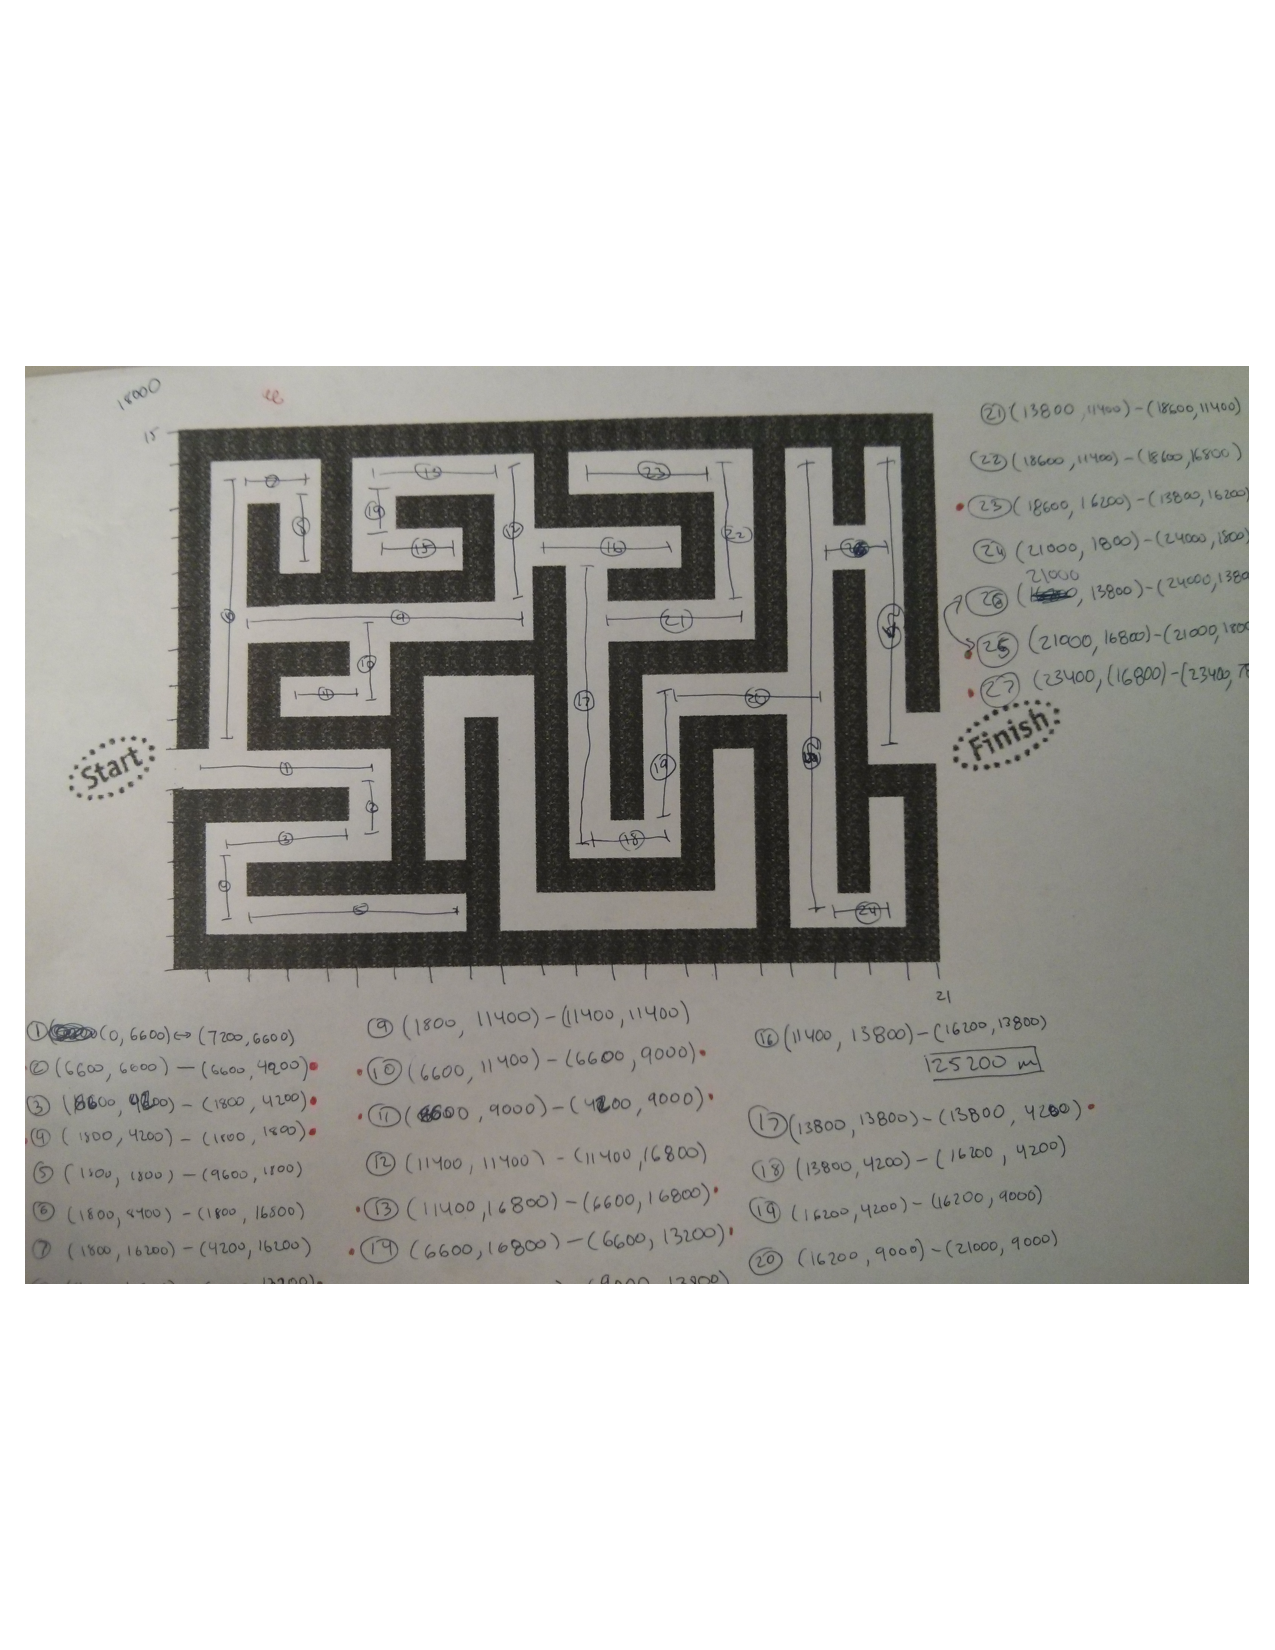
\includegraphics[width=.9\columnwidth]{figures/maze.pdf}
\end{center}
\caption{The maze!}
\label{fig:maze}
\end{figure}

% -----------------------------------------------
%   The Oil Spill!
% -----------------------------------------------
\subsection{The Oil Spill!}


% -----------------------------------------------
%   The Volcano!
% -----------------------------------------------
\subsection{The Volcano!}


% -----------------------------------------------
%   The Sharknado!
% -----------------------------------------------
\subsection{The Sharknado!}



